% !TEX encoding = UTF-8 Unicode
\documentclass[11pt]{article} % use larger type; default would be 10pt

%%% PAGE DIMENSIONS
\usepackage{geometry} % to change the page dimensions
\geometry{a4paper} % or letterpaper (US) or a5paper or....


%%% PACKAGES
\usepackage[utf8]{inputenc} % set input encoding (not needed with XeLaTeX)
\usepackage{subfiles}
\usepackage{amssymb}
\usepackage{tabulary}
\usepackage{color, colortbl}
\usepackage{xcolor}


\usepackage{graphicx, wrapfig} % support the \includegraphics command and options

\DeclareGraphicsExtensions{.png,.jpg}
\graphicspath{{img/}{../img/}}
\usepackage{gensymb}
\usepackage{pdfpages}
\usepackage{standalone}
\usepackage{float}
\usepackage[toc,page]{appendix}

%%% Codes
\usepackage{listings}
\definecolor{Gray}{gray}{0.9}
\setlength{\parindent}{0em} 

\usepackage[breaklinks=true]{hyperref}


%%% HEADERS & FOOTERS
\usepackage{fancyhdr}	% This should be set AFTER setting up the page geometry
\pagestyle{fancy}	% options: empty , plain , fancy
\renewcommand{\headrulewidth}{0pt}	% customise te layout...
\lhead{}\chead{}\rhead{}
\lfoot{}\cfoot{\thepage}\rfoot{}

%%% END Article customizations

\begin{document}

\begin{titlepage}
    \begin{center}
        \vspace*{1cm}
        
        \Huge
        \textbf{IP5}
        
        \vspace{0.5cm}
        \LARGE
        Snow Uber - A context aware C2C mobile app
      
        \vspace{1.5cm}
        
        \textbf{Author: Lukas Schönbächler, Tobias Ernst}\\
        \textbf{Supervisor: Thekla Müller, Jürg Luthiger}\\
        \textbf{Client: papers.ch, Alessandro De Carli}

		\vspace{1.5cm}        
        
        
\includegraphics[width=0.8\textwidth]{title/title}
        
        \vfill
        
       
        \vspace{0.8cm}
        
        
\includegraphics[width=0.4\textwidth]{title/fhnw}
        
        \Large
        IMVS\\
        University of Applied Sciences and Arts\\
        Switzerland\\
       January 20, 2017
        
    \end{center}
\end{titlepage}

\begin{abstract}
The goal of this work is to develop an app prototype with its backend to improve the visibility of private snow sport teachers (ski and snowboard) in order to reduce the high price situation in ski-regions. This work consists of two parts. The first part describes the architecture of the end user application as well as the corresponding backend to it. The second part focuses on an additional separate module called “rule engine”, developed to empower users to use reported data for marketing campaigns, such as sending an email when a user enters a specified area or notifying users about a discount when the weather is bad.
\end{abstract}

\newpage
\tableofcontents
\newpage

\section{Introduction}
Ski schools claim high profit margins from their teachers. Since this business is seasonal by its nature and the personnel is paid hourly, we had the idea to privatize their services. The model is similar to Uber or Airbnb: A person offers a service and another person can consume this service through the platform.\\
The whole matching and organizing process should be done through the app. A rating system should help to assure quality and build a community around it.
\newpage

\section{Objectives}
During the kick-off meeting, our advisors pointed out, that it will be required to focus on one particular technical aspect and go in depth of this topic. To evaluate this topic, we came up with the following matrix:

\vspace{0.5cm}
\begin{tabulary}{\linewidth}{LLL}
    \hline
    Topic&+&-\\
    \hline
Security&&Not a key feature in this business\\
Payment&&Achievable through numerous APIs\cite{payment-apis})\\
Performance&&Not a key feature in this business, not through non-native apps\\
AI (i.e. Chatbot)&Interesting topic, marketing relevant&Out of scope, maybe for IP-6\\
\rowcolor{Gray}
Context aware notifications  (sensor, rule engine)&Interesting topic, marketing relevant& \\
Usability&Interesting topic, marketing relevant&Different field of specialization\\
    \hline
\end{tabulary} 

\vspace{0.5cm}
We decided to focus on context awareness. The organization should be able to create customized process chains to target their customers in a personal way.\\
To achieve this, the goal of this project is to develop two parts:

\begin{itemize}
  \item An application which provides basic functionality such as browsing through offers, booking a service and chatting with the teacher. While doing these actions, the app should emit actions to the rule engine, such as user creation, geofence entered, booking created etc.
  \item A web interface which lets organizations configure their recipes to target their customers in a personal way.
\end{itemize}

Therefore, the application requires a backend to create offers and manage bookings. This will be generated by the default Django Framework and will be customized to just display the data relevant to the current authenticated user. Nevertheless, it is not the main scope of this project. Since this will be a prototype, it will not be released in any app store as long as there are no partners. Instead our project customer will contact a few ski school individually and sell the solution to them directly, after building this initial selection of partners, the app will be released.

\newpage

\section{Overview}

Technology wise, the project can be divided into four parts:

\begin{itemize}
  \item Mobile Application: Ionic 2
  \item Mobile Backend: Python with Django
  \item Rule Engine: Angular 1 with Typescript
  \item Rule Engine Backend: Python with Django
\end{itemize}

\newpage

\section{Mobile app}
\subsection{Technology}
The products success depends on its wide spread user base. Because of this, it is important to make the frontend part available to as many users as possible. For this reason, the customer asked for a cross platform application, which allows him to maintain all the functionalities in one unified code base.\\
Fortunately, this requirement can be solved by various technological solutions at the time. Namely those are:

\begin{itemize}
  \item Ionic\cite{ionic} - an open source mobile SDK for developing native and progressive web apps (Typescript/JavaScript)
  \item React native\cite{react-native} - an open source library to compile native component code from JavaScript
  \item Xamarin\cite{xamarin} - Cross compiler platform for iOS Android and Windows Phone(C\#)
\end{itemize}

The decision ultimately was done by the help of the following comparison matrix:

\vspace{0.5cm}

\begin{tabulary}{\linewidth}{LLLL}
    \hline
    Feature&Xamarin\cite{xamarin}&Reactive Native\cite{react-native}&Ionic 2\cite{ionic2}\\
    \hline
	Customer requirements (Geofence, iBeacon)&Covered&Covered&Covered\\
	Crossplatform compatiblity&Android, iOS, Windows Phone 8&Android, iOS&Android, iOS, Browser (Progressive Web App)\\
	Existing knowledge&None&Sparsely&Good\\
	Maintainability&Good&Good&Good\\
	License / Pricing&MIT / open source&BSD License&MIT / open source\\
	Futureproof&Yes / Supported by Microsoft&Yes / Supported by Facebook&Yes / Supported by Google\\
    \hline
\end{tabulary} 

\vspace{0.5cm}

We ended up using Ionic 2, mainly because of the existing knowledge, but also due to the fact that it is a powerful framework including components\cite{ionic2} covering most of our needs out of the box.
\newpage
\subsection{Functionality}
\subsubsection{Login Page}
Before the user is allowed to interact with the app, he needs to sign up. The user is redirected to the registration page on the initial app start.\\
A email and password is required to register as a new user. If an input is missing or wrong (i.e. no valid email address), the register button remains disabled. The user accepts the general terms and conditions by clicking on “register”. After a successful signup, the user will be redirected to the main screen. 

\subsubsection{Menu}
The app contains a tabbed menu with four pages

\begin{itemize}
  \item Browse
  \item Map
  \item Messages
  \item Profile
\end{itemize}

\subsubsection{Browse}
The initial screen shows a list of available offers. The offers can be sorted by rating, price or location. The location filter sorts the list by the relative position of the user to an existing offer. If a user moves around, the list will update simultaneously. By pressing on an offer, the detail view will show up.

\subsubsection{Map}
Available offers can be shown in a map view. A pin indicates the user's current location. Offers are represented by a colored area. By pressing on the area, the tab will switch back to the browse view and the list is filtered to the selected region.

\subsubsection{Offer detail}
The offer detail page shows all important information, such as price, duration and much more. It enables the user to book an offer.  The following actions are possible:\\

\begin{itemize}
  \item Click on an organization's name, the company's profile page is shown.
  \item Click on the book button to book an offer. More information is needed to send the booking request.
 \item The chat button allows to chat with the organizations responsible in order to ask get more detailed information.
 \item Rate an offer: A user can rate an offer after it was booked and the organization confirmed the it.
\end{itemize}

\subsubsection{Organization’s profile}
The company's profile page contains general information about the organization such as a small descriptive text,, the address and the contact person.

\subsubsection{Create an order}
When creating an order, the user gets a list with available dates from which he can choose one or several. This list is generated through minimum information like date from, date to, weekdays and duration, which are set in an offer by the organization. Possible durations are: morning, afternoon or full day. We wanted to design the booking process as easy and transparent as possible, that is why the user does not get a date picker but only a list with available dates. 

\begin{figure}[H]
\begin{center}
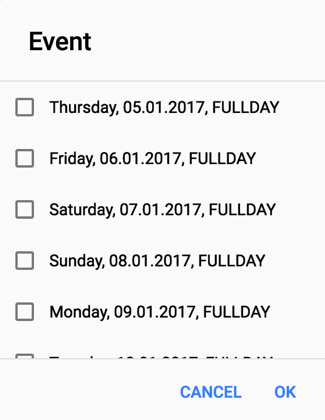
\includegraphics[]{event_creation}
\end{center}
\caption{Date selection dialog when creating a booking}
\label{fig:event_creation}
\end{figure}
\newpage
To visualize the whole process, we created an activity diagram:
\begin{figure}[H]
\begin{center}
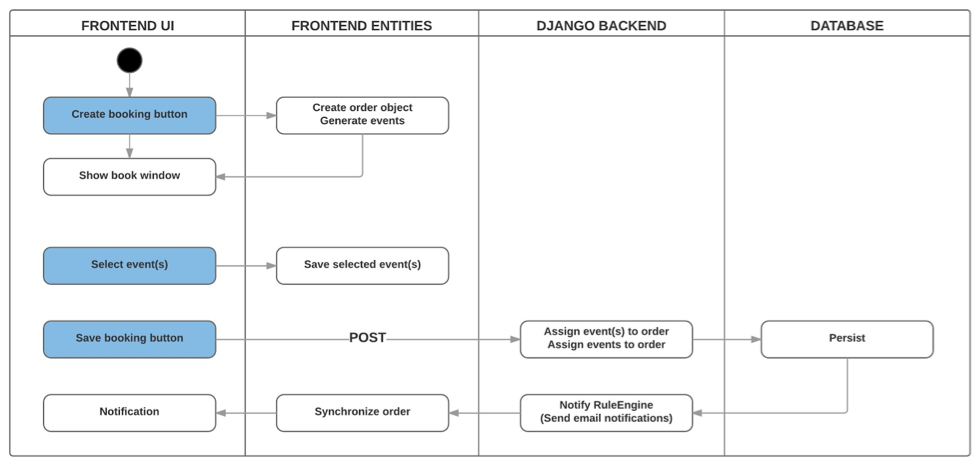
\includegraphics[width=1.0\textwidth]{order_post_activity_diagram}
\end{center}
\caption{Create order activity diagram}
\label{fig:order_post_activity_diagram}
\end{figure}


\subsubsection{Change an order}
A user can change a booking as long as it is not confirmed by the organization. The events are fetched from the backend. Because the available events are generated by the frontend, an event has no unique identifier. Therefore, the ion-select component identifies and pre-selects all existing events from the existing order by a hash code which is generated by the event’s date and duration.

\begin{figure}[H]
\begin{center}
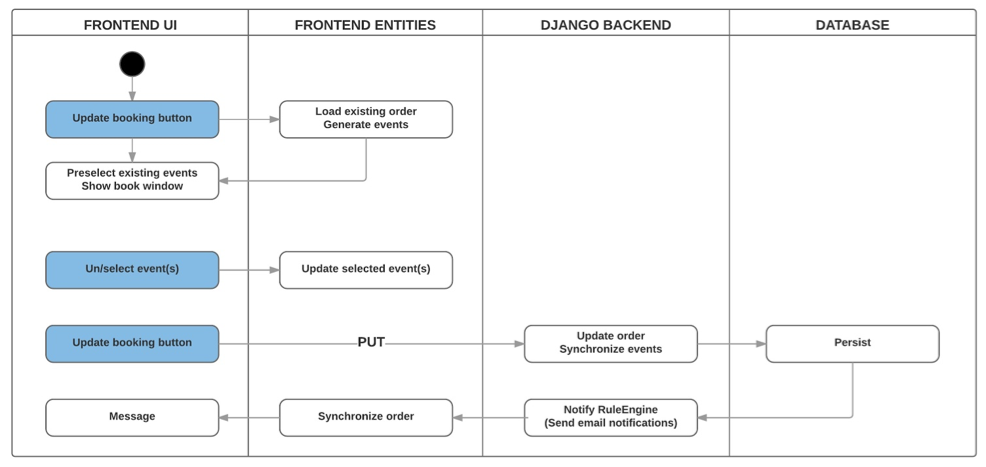
\includegraphics[width=1.0\textwidth]{order_put_activity_diagram}
\end{center}
\caption{Update order activity diagram}
\label{fig:order_put_activity_diagram}
\end{figure}


\subsubsection{Delete an order}
An order can be cancelled as long as the offer’s organization did not confirm it. The cancel button is only available if a cancellation is possible.

\begin{figure}[H]
\begin{center}
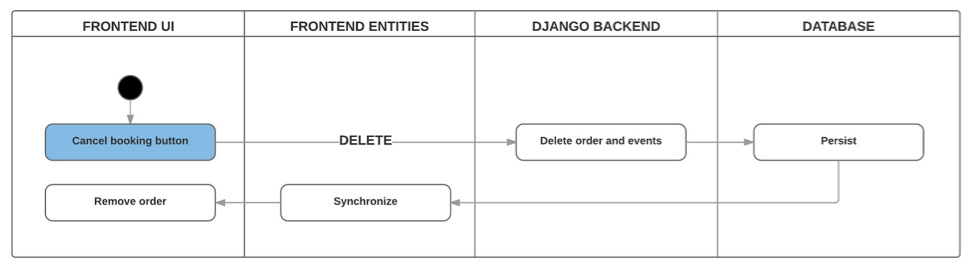
\includegraphics[width=1.0\textwidth]{order_delete_activity_diagram}
\end{center}
\caption{Delete order activity diagram}
\label{fig:order_delete_activity_diagram}
\end{figure}

\subsubsection{Messages}
Messages are similiar to almost all chat applications. It allows the user to interact with the company’s contact person. Communication is always between two people. The message screen contains the message history. A user can write new message by entering the text into the textbox and sending it by clicking on the send button. The chat module allows to write simple text without any kind of formatting functionality. It also allows the user to share personal information such as his phone number or email address. 

\subsection{Technical aspects}
\subsubsection{Http service}
Our app is mainly doing backend requests to the Django backend which is persisting all data. The communication is done with the help of the Angular 2 http service, which returns an observable or a promise object.\\
Our service implementation holds a user object with all the necessary information required to authentificate agains the backend. All the communiation is done trough https, which means it is end to end encryptend. Except of the registration or the login endpoint, all the requests are authorized by a token\cite{djoser}. Some responses are  filtered by Django based on the authenticated user, therefore the ionic 2 frontend does not have to care about information that should not be shown to a user. Such filtered information are for example chat messages or orders.

\subsubsection{User Management}
After sending initial credentials to the server an authentication token is returned and stored in the local storage of the browser. An instance of the user object is saved as a part of the http provider implementation. The authentication token is attached to each backend request afterwards.

\subsubsection{Multi language}
Since the application is primarily target user group are tourists, it is important to provide different languages. Therefore the whole application is translated with the help of ng-translate\cite{ng-translate}, the official i18n internationalization library. A new language can be added by translating the en.json file in the assets folder and name it in the locale it is translated. The base language of our app is English, but we also translated it to German as well. The library automatically selects the devices locale language if available, otherwise it uses the fallback language which is as already mentioned English.

\subsection{Context awareness}
To achieve context awareness, we need to consider which information are relevant for our use case. Today's smartphones have a wide variety of sensors. Since we decided to use ionic 2, we did some research and found the official cordova plugin to interact with the devices sensors:\\

https://github.com/fabiorogeriosj/cordova-plugin-sensors\\

Their documentation unveils all sensors available on modern smart phones:\\

\vspace{0.5cm}

\begin{tabulary}{\linewidth}{LL}
    \hline
    Sensor&Description\\
    \hline
	PROXIMITY                     & Measures the proximity of an object in cm relative to the view screen of a device.\\
	ACCELEROMETER                 & Measures the acceleration force in m/s2 that is applied to a device on all three physical axes (x, y, and z), including the force of gravity. \\
	GRAVITY                       & Measures the force of gravity in m/s2 that is applied to a device on all three physical axes (x, y, z).\\
	GYROSCOPE                     & Measures a device's rate of rotation in rad/s around each of the three physical axes (x, y, and z).\\
	GYROSCOPE\_UNCALIBRATED       & Rate of rotation (without drift compensation) around the x axis.\\
	LINEAR\_ACCELERATION          & Measures the acceleration force in m/s2 that is applied to a device on all three physical axes (x, y, and z), excluding the force of gravity. \\
	ROTATION\_VECTOR              & Measures the orientation of a device by providing the three elements of the device's rotation vector.\\
	STEP\_COUNTER                 & Number of steps taken by the user since the last reboot while the sensor was activated.\\
	GAME\_ROTATION\_VECTOR        & Rotation vector component along the x axis.\\
	GEOMAGNETIC\_ROTATION\_VECTOR & Rotation vector component along the x axis.\\
	MAGNETIC\_FIELD               & Measures the ambient geomagnetic field for all three physical axes (x, y, z).\\
	MAGNETIC\_FIELD\_UNCALIBRATED & Geomagnetic field strength (without hard iron calibration) along the x axis.\\
	ORIENTATION                   & Measures degrees of rotation that a device makes around all three physical axes (x, y, z).\\
	AMBIENT\_TEMPERATURE          & Measures the ambient room temperature in degrees Celsius. See note below.\\
	LIGHT                         & Measures the ambient light level (illumination) in lx.\\
	PRESSURE                      & Measures the ambient air pressure in hPa or mbar.\\
	RELATIVE\_HUMIDITY            & Measures the relative ambient humidity in percent (\%).\\
	TEMPERATURE                   & Measures the temperature of the device in degrees Celsius.  \\
    \hline
\end{tabulary} 

\vspace{0.5cm}

Even though this list may look impressive, we have to put this into the right context. There are four main problems:

\begin{itemize}
  \item Relevance - Many of these sensor data are just not relevant at all
  \item Availability - Only few devices actually provide these sensors, this list just shows what the systems may deliver (i.e. a small research on gsmarea.com showed us that only 11 out of 7944 devices actually implemented a temperature sensor)
 \item Accuracy - I.e. if you want to use the temperature data together with the humidity data to predict the weather, it’s crucial where the device actually is, if the owner is inside the house, the measurement is useless
 \item Battery impact - The more and often we use a sensor, the more we drain the battery. Especially in a cold environment like the mountains this is counterproductive. People will uninstall the app if they see that it drains battery in the background by pulling sensor data and sending it to our server
\end{itemize}

As you see, most of the devices sensors are probably useless. Our use cases are mostly related to the location. A basic example could be:\\

\colorbox{blue!30}{A user should automatically receive an email with a rabatt code}
\colorbox{green!30}{when he arrives at the ski resort}
\colorbox{orange!30}{and}
\colorbox{red!30}{ and the weather is bad.}\\

This can be divided into the following parts:\\

\colorbox{blue!30}{  } Action that has to be taken in case the premise was fulfilled\\
\colorbox{green!30}{  } Condition 1: Event triggered by location\\
\colorbox{orange!30}{  } Conjunction\\
\colorbox{red!30}{  } Condition 2: Abort in case the weather is not bad\\

As you can see, we somehow need to know the location and the weather at the given location. The location part is not a big deal, the best way to do this, is to use geofences.

\subsubsection{Geofences}
As the name suggests, geofences are basically virtual fences. They empower you to create digital boundaries which will notify you whenever you cross them. To accomplish this, geofences use all sorts of sensors together to improve accuracy while reducing the battery drain, it uses GPS, Wi-Fi and Bluetooth combined. It’s a passive solution, which means in order to create a geofence, there is no hardware required.

\begin{figure}[H]
\begin{center}
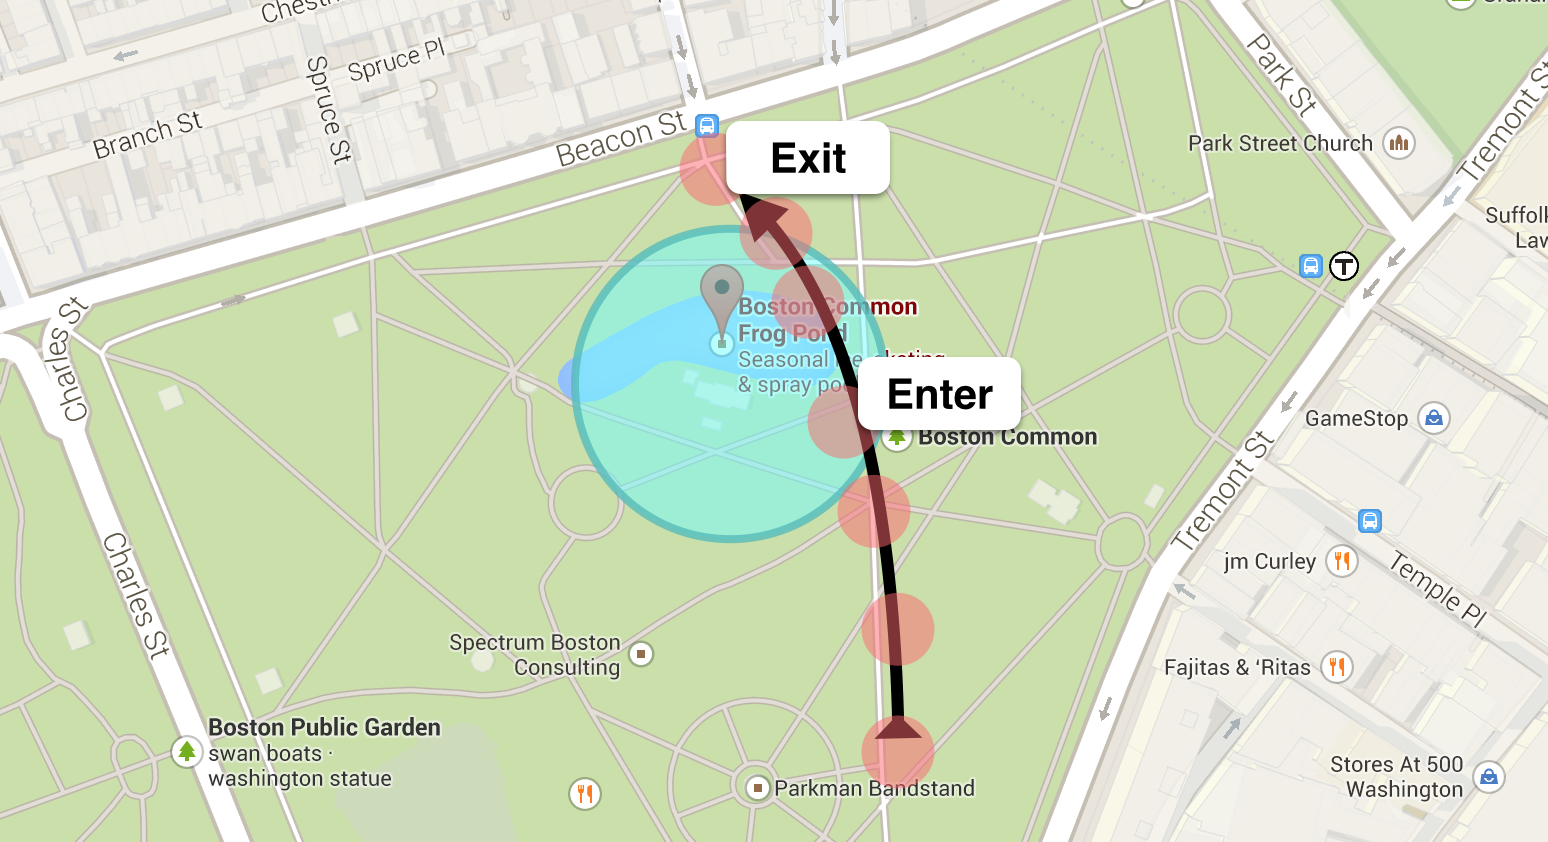
\includegraphics[width=1.0\textwidth]{geofences}
\end{center}
\caption{Example how when geofence\cite{geofence} events are triggered}
\label{fig:geofences}
\end{figure}

On modern smartphones running Android or iOS, there is a system wide service where you can submit a geofence or subscribe to one. After subscribing, your listener will be called, whenever you enter or leave the fence. The system will take care of all the other parameters, it will schedule when it has to check the next time or it will take care of what happens if you deactivate GPS for example. This system wide scheduling helps to prevent the battery from draining too fast.

\subsubsection{Weather data}
Since we now have the location of a user, we pull weather data from an open API. This could be done on the phone, but to save battery, it is more convenient to do it in the backend. Therefore, it is enough, if we just send the coordinates (or even the place ID of the geofence we were listening to) to the server.

\subsubsection{Location service implementation}
There are at least three different cordova plugins available that are implementing geofences. But they all work in a different way. It is worth mentioning the fact that using web technology is a huge limitation in most cases. Since geofences are managed by the system\cite{geofence-android}, the listener has to be native code. In consequence, the following plugins have to register a native listener and since it is not possible to run a browser context in a background thread, we are limited to predefined actions provided by the plugins listener.\\

\textbf{cordova-plugin-geofence}\cite{cordova-plugin-geofence}\\
This plugin is the one supported by the ionic community. It supports the latest version of Android, Windows Phone 8 as well as iOS. You can configure it to show a notification or to vibrate whenever a geofence is entered or left. As soon as the user clicks on the notification, our attached JavaScript listener gets triggered and our custom logic executed. Unfortunately, this means, that in order to trigger an action, the user has to click on the notification.\\

\textbf{phonegap-geofencing}\cite{phonegap-geofencing}\\
This one is similar to the Cordova-plugin-geofence, but without the Windows Phone 8 support. It also looks like it is not supported any longer.\\

\textbf{cordova-plugin-background-geolocation}\cite{cordova-plugin-background-geolocation}\\
Even though the name implies that this plugin is related to geofences, it actually creates a background thread. Instead of showing the user a notification, it is possible to pass an URL to the listener. Whenever the location changes, the listener posts the new location information to this URL. It even stores the locations to send them later, in case there is no active internet connection.\\

\textbf{cordova-background-geolocation-lt}\cite{cordova-background-geolocation-lt}\\
After a lot of searching, we stumbled upon this plugin. It works in a similar way as the Cordova-plugin-background-geolocation, but it actually uses the geofencing service. It even allows monitoring infinite geofences instead of max 20 on iOS or 100 on android. It’s highly configurable, well documented and very power efficient. The only downside is, that it costs 300\$ for the android version (the iOS version is available for free).\\

We decided to use this plugin for the prototype. In case this project will go to production 300\$ is not that much of an investment. Especially, after comparing the quality of the documentation, response time on issues and after comparing functionality and reliability.\\
\newpage
Therefore, our geofence process ended up looking like this:

\begin{figure}[H]
\begin{center}
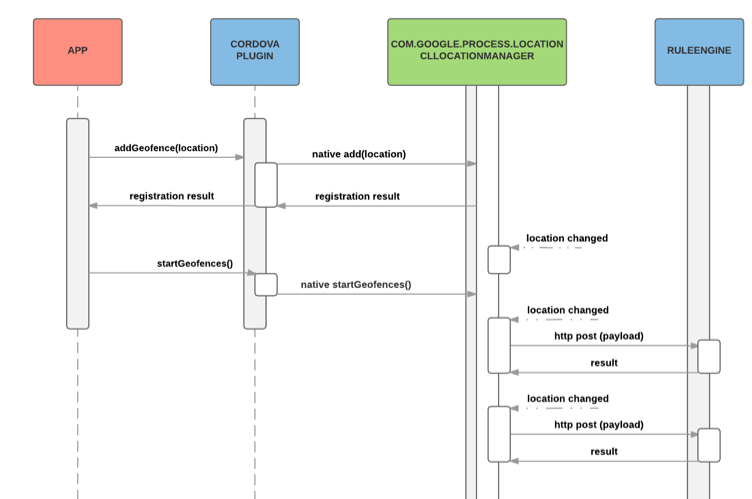
\includegraphics[]{geofence_process}
\end{center}
\caption{Geofence triggered by the cordova plugin}
\label{fig:geofence_process}
\end{figure}

\vspace{0.5cm}


Important is the fact, that even if the application is closed (i.e. if the device was restarted), the registered geofences are still monitored and location change events are reported back to the rule engine by a post request. Since this part was done through a native Cordova plugin, there is no need for a browser context which could run injected JavaScript code. The biggest advantage compared to a background service is, that the user is not able to kill the process, without affecting his whole system.\\

\textbf{Conclusion}\\

Even though modern devices potentially provide a wide variety of sensors, most of them ended up not being useful in our scenario. The only interesting sensor was the user’s current position. Gathering this information in real time in a hybrid app, ended up being more difficult than we anticipated in the beginning, especially when battery usage is important. While testing all the plugins, we noticed that most of them were of bad quality, the documentation was outdated or it didn’t run at all. This really surprised us, especially due to the fact that geofences are used in a lot of popular apps. The plugin we eventually ended up with, was a complete different story, but this is probably due to the fact, that this guy makes good money with it.

\subsection{Token Based Authentication}
When sining up a user by email and password, Django creates an authentication token and stores it in the database. The Ionic frontend on the other side retrieves the authentication token after a successful login and remembers it by adding the token into the local storage.\\
Authentication tokens can be invalidated by truncating the authtoken table of the database.\\
The registration and login request contain the plaintext user password. For that reason, we use a secure https connection for registration and login process.

\subsection{Registration/Login}
Django authorizes a user by his email address. A backend entity “Person” inherits from “AbstractBaseUser” which allows Django to handle user credentials. Moreover, we implemented our own UserManager to tell Django to use an email address instead of an username.\\
Below, you can see an activity diagram that explains the complete process.

\begin{figure}[H]
\begin{center}
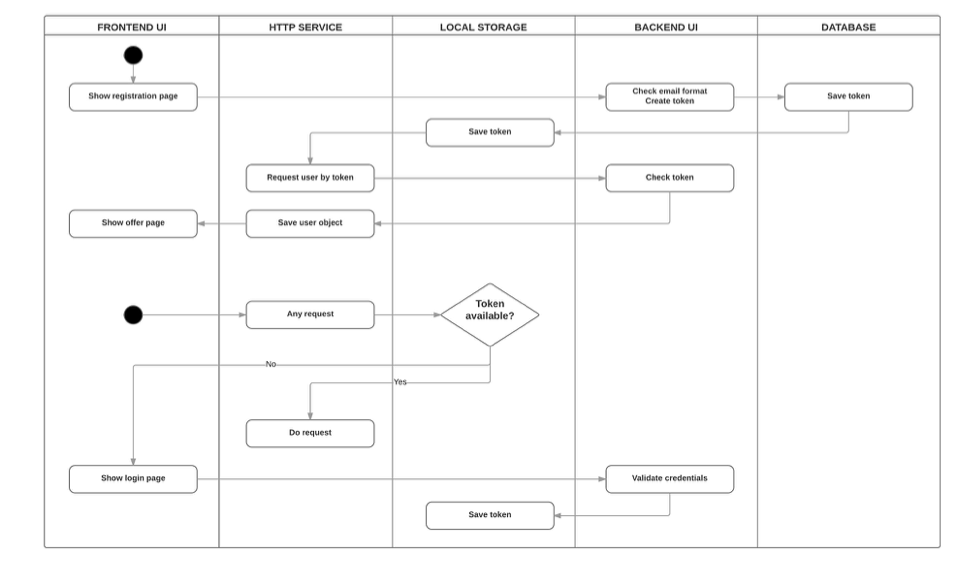
\includegraphics[]{registration_process}
\end{center}
\caption{User registration process activity diagram}
\label{fig:registration_process}
\end{figure}



\section{Django Backend}
\subsection{Technology}
The backend technology was up to us, the customer just mentioned that he already had a productive environment for Django applications. We did not have any knowledge with this framework at that time, but after doing the first sample, we were convinced that we were able to acquire the knowledge needed in order to successfully complete this project. The other big option was Spring Boot.\\

\begin{tabulary}{\linewidth}{LLL}
    \hline
    &Spring Boot/Java      & Django/Python                         \\
    \hline                            
Customer requirements & Possible       & Preference             \\
Backend UI            & Plugin         & Built-In               \\
Existing knowledge    & Yes            & No                     \\
Maintainability       & Good           & Good / highly scalable \\
License / Pricing     & Apache License & BSD License      \\     
    \hline
 \end{tabulary} 
 
 \vspace{0.5cm}

 
Python is dynamically typed as default. This makes debugging and error handling more difficult. Nevertheless, we decided to use python mainly because there is a customizable backend UI. Furthermore, our customer preferred this technology. We learned Django and Django Rest Framework (DRF) by working through the documentation\cite{django} which is informative and well explained.

\subsection{Models}
The Ionic frontend and the Django backend application contain several entities to synchronize data. There are small differences between backend and frontend models.\\

First, Django lets us use a custom “DateField” but the Ionic app needs the dates in a string format for the date picker. Moreover, methods are defined where they are needed. For example, the frontend model “Offer” contains a method “generateEvent” and all backend models contain a “\_\_str\_\_” (toString) method which are required by the Django backend UI.\\


\subsubsection{Allowed methods}

\begin{tabulary}{\linewidth}{LLLLL}
    \hline
    Entity& POST  & PUT   & GET   & DELETE \\\\
    \hline                            
Place                       & No    & No    & Yes * & No     \\
Person                      & Yes * & Yes * & Yes * & No     \\
Organization                & No    & No    & Yes   & No     \\
Offer                       & No    & No    & Yes   & No     \\
Order                       & No    & Yes * & Yes * & Yes *  \\
Rating                      & Yes * & No    & No *  & No     \\
Message                     & Yes   & No    & Yes   & No     \\
Country                     & No    & No    & Yes   & No     \\
Currency                    & No    & No    & Yes   & No     \\
Language                    & No    & No    & Yes   & No     \\
Sport                       & No    & No    & Yes   & No     \\
Event                       & No    & No    & No    & No    \\
    \hline
 \multicolumn{5}{l}{* means: partially possible under preconditions described below}
 \end{tabulary} 
 \\
 \subsubsection{Abstract Component}
We tried to keep the models flat, but in the end, each entity inherits from AbstractComponent. A simple base class with a date created and a date modified timestamp. If a model does not contain an explicit primary key, Django creates unique identifier on its own.

\subsubsection{Person}
A person is a customer. The class contains some basic information which we use later for the billing. Furthermore, it contains information about sports a user wants to learn. This information can be used in the rule engine afterwards.\\
The Person POST request is used to create a new account. The PUT request is to update an existing profile. The Person which is fetched by the frontend app doesn’t contain information from AbstractBaseUser, which is important for security.

\subsubsection{Organization}
Each organization is represented by a default person which is responsible for the customer communication (chatting). Such a person can edit offers and change booking states over the Django Backend UI.\\
An organization holds a list of offered sports, so that the user can see this information on the organization's profile page.\\
The Organization model is extendable with possible workers (teachers). Later, workers should be able to create offers without an organization behind.

\subsubsection{Offer}
Offers can only be created in the Django Backend UI. Each offer can be booked from a person only once. 

\subsubsection{Order}
An order can contain several events. The possible event dates are generated out of several parameters as described in the frontend part of this document. \\
Updating and deleting an order is only possible if the order status has not been confirmed so far. An order is a personal property. That means it is bound to a person. The GET request only returns orders that belong to the requesting user.

\subsubsection{Place}
Each place contains coordinates and a radius to cover an area. A place represents for example a ski resort or a tourist attraction. Places are important for the geofence service. The map layout uses places to visualize the closest offer of the current location.\\
We use get requests on the “Place” entity for the geofence service. Places have to be registered once, so that events can be triggered on location entry or exit. 

\subsubsection{Rating}
The customer can give a rating for each order he booked. It would be useful to rate exclusively the booked teacher, but the offer is bound to an organization (school e.g.) and not to a teacher directly.\\
It is only possible to give a rating until the organization has confirmed the order (booking). Ratings let us calculate the organization's average rating and the offer's average rating. Rating values are represented through stars on the “Offer page”.
\newpage

\subsection{Permissions and security}
We allow several ways to interact with Django. First, over Django Rest Framework (DRF) mentioned above and second over the built-in Django backend which is well customizable.\\
We customized the backend as followed:\\

\begin{tabulary}{\linewidth}{llllllllll}
    \hline
    Django Backend UI &                   &        &        &               &        &        &                      &        &        \\
                  & \multicolumn{3}{c}{Backend Superuser}           & \multicolumn{3}{c}{Backend Staff}    & \multicolumn{3}{c}{Backend Default User}          \\
                  & C            & U & D & C        & U & D & C               & U & D \\
    \hline                            
Place             & Yes               & Yes    & Yes    & No            & No     & No     & No                   & No     & No     \\
Person            & Yes               & Yes    & Yes    & No            & Yes *  & No     & No                   & No     & No     \\
Organization      & Yes               & Yes    & Yes    & No            & Yes *  & No     & No                   & No     & No     \\
Offer             & Yes               & Yes    & Yes    & Yes           & Yes *  & Yes *  & No                   & No     & No     \\
Order             & Yes               & Yes    & Yes    & Yes           & Yes *  & No     & No                   & No     & No     \\
Rating            & Yes               & Yes    & Yes    & No            & No     & No     & No                   & No     & No     \\
Message           & Yes               & Yes    & Yes    & No            & No     & No     & No                   & No     & No     \\
Country           & Yes               & Yes    & Yes    & No            & No     & No     & No                   & No     & No     \\
Currency          & Yes               & Yes    & Yes    & No            & No     & No     & No                   & No     & No     \\
Language          & Yes               & Yes    & Yes    & No            & No     & No     & No                   & No     & No     \\
Sport             & Yes               & Yes    & Yes    & No            & No     & No     & No                   & No     & No     \\
Event             & Yes               & Yes    & Yes    & No            & No     & No     & No                   & No     & No      \\
    \hline
 \end{tabulary} 
 
 \vspace{0.5cm}
 
 Django pre-defines three user groups: “Superuser”, “Staff” and “Default”. A super user can perform all actions. He has full control. The default user has no permissions to login to the backend. Each organization user is a staff user. Organizations and the organization's default person is linked manually at the moment. This means a super user must login to the admin panel and create an organization. After that, a default person is linked.\\
 \\
Django offers group permissions. We set up such a group to share basic permissions to organization users. An organization user may edit offers, orders, persons and organizations.\\

\begin{figure}[H]
\begin{center}
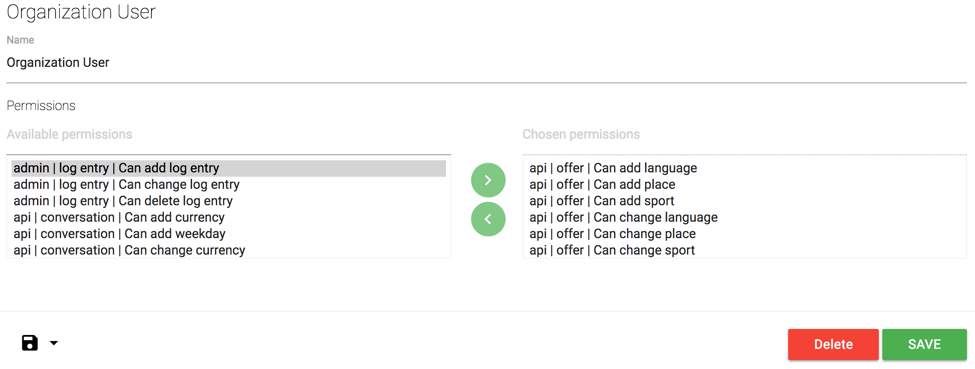
\includegraphics[width=1.0\textwidth]{group_permissions}
\end{center}
\caption{Django group permissions}
\label{fig:group_permissions}
\end{figure}

These entities are quite not customized. This means a staff user can only edit foreign organizations, orders and offers and his own profile. Moreover, we restricted access to some fields like the ID or some other read only fields, which don’t affect the business.\\
\\
Customized entities are marked with a star (*) in the table above. The filter is always set with the currently logged in user.

\newpage
\section{Ruleengine}
\subsection{Introduction}

One big part of the product is a backend functionality called the rule engine. It enables the administrator to automatically trigger actions depending on certain data. Some examples are:

\begin{itemize}
  \item Send an email to a user on his birthday
  \item Send an email to a user when he entered a ski region
  \item Send a sms to a user when tomorrow's weather is good
  \item Send a welcome email when a new user is registered
\end{itemize}

Organizations should be able to configure the parameters by a few clicks and adjust these “recipes” through an intuitive UI. It is also important to make this system as flexible as possible, it should be able to extend its functionality by adding a few lines of code.

\subsection{Technology}
In the beginning, we thought this was a no brainer. Due to the fact that Ionic 2 was based on Angular 2, we started implementing it with Angular 2. Unfortunately, it turned out that Angular 2 was not ready to fulfill our needs at the time. We were missing basic components, faced various bugs and eventually switched to Angular 1 with Typescript.\\
\\
The "rule engine" backend is programmed in Django as we used Django already for the app backend.

\subsection{Components}
There is a well-known service called “If This Then That” or short www.ifttt.com\cite{ifttt} , which do offer the kind of functionality we need in a limited way. To use their service, you must register and afterwards you can create new “recipes”. These recipes are a composition of two components, a trigger and an action. Unfortunately, this approach isn’t flexible enough to fulfill our use cases and therefore we came up with a more complex process chain. It looks as following:

\begin{figure}[H]
\begin{center}
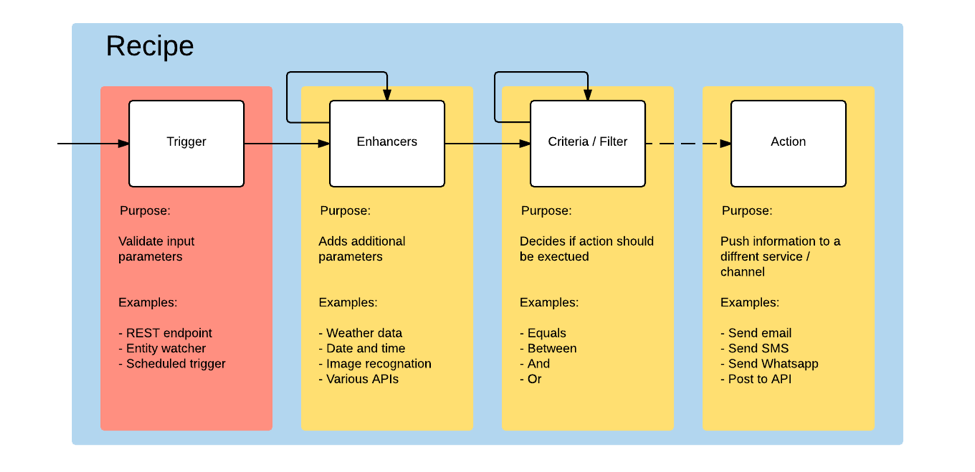
\includegraphics[width=1.0\textwidth]{recipe_process}
\end{center}
\caption{Recipe process}
\label{fig:recipe_process}
\end{figure}

Beside the trigger and the action (which are more or less identically to their counterparts from ITTT), we also introduced components called enhancers and criterias. These additional components empower the user to enhance a request with additional information (i.e. weather data depending on the provided location) and allow him to afterwards terminate the process chain before an action gets executed (i.e. if the weather temperature is above 10C).\\
\\
There is a downside caused by this additional functionality - it’s a lot more performance intensive than a simple input / output approach. Whenever a recipe gets triggered, numerous enhancers and filters get executed, which increases the duration to evaluate the whole chain. Caused by this circumstance, we implemented the trigger in a “hit and run” kind of matter. Whenever a trigger gets triggered, all the necessary parameters get validated (red) and the validation result is reported back to the requester immediately. This does not mean the action was triggered, it just means that the request was valid and is queued up in the rule engine worker queue. All the remaining parts of the chain afterwards run in a new worker thread (yellow). Therefore we use a job scheduling library called celery\cite{celery}, which provides a pool of workers. If needed, new workers can be connected to this pool. In case all workers are busy when a new task is submitted, it automatically persists the task and loads it as soon as a worker becomes available.\\
\\
Between one component and the next exists a contract which validates the passed parameters each time the border is crossed in order to guarantee defined preconditions to the concrete implementation parts. This also enables us to suggest placeholders to the user or to display available fields in the filter list. Furthermore it enables us to enforce advanced logging to report faulty input to the user with many additional information.\\
\\
We will now explain the different components in detail:

\subsubsection{Triggers}
The triggers main function is to validate or gather the parameters they provide according to their contract. It is possible that a trigger requires additional configuration (fields will show up when you create a recipient). There are two types of triggers, periodic and non-periodic ones.\\

\textbf{Periodic}\\
Periodic triggers are, as the name already presumes, triggers which are called in a periodic interval. They can be scheduled in the same way as crontabs are scheduled:

\begin{figure}[H]
\begin{center}
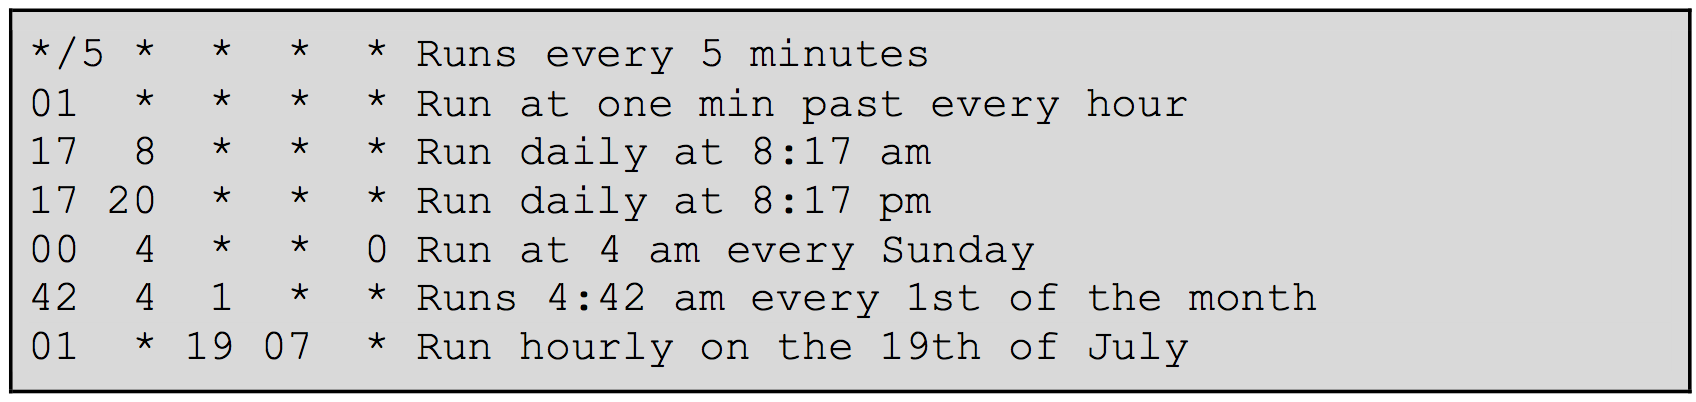
\includegraphics[width=1.0\textwidth]{cron}
\end{center}
\caption{Scheduling examples}
\label{fig:cron}
\end{figure}

Whenever a periodic trigger gets executed, the custom logic gathers all parameters (i.e. through a SQL query), loads all subscribed recipes and creates a new task which afterwards gets pushed into the worker’s queue.\\
\\
\textbf{Non-periodic}\\

Non periodic triggers are triggered manually either through a web service call or by listening to a database event (i.e. new user created). Similar to the periodic triggers, the non periodic trigger has to guarantee that all defined contracts are fulfilled, otherwise, the event will be rejected and logged.

\subsubsection{Enhancers}
Enhancers can add additional information depending on the passed input parameters. As example, it is possible to look up weather data depending on the passed location. Therefore, the “WeatherEnhancer” requires a location parameter, which will be used to query the data from an external service such the openweather\cite{openweather} API. These parameters will be added to the existing parameter set and can be used as input parameter for other enhancers or can be used to filter afterwards. Based on the selected trigger, the frontend automatically calculates which enhancers can possibly be added and then adds them during the recipe creation. This calculation can be done recursively: We add enhancers as long as we fulfill their contract and remove them from the list of available enhancers. Whenever an enhancer has been added, we have to go through the whole remaining list again (since adding a new enhancer implies having more parameters than in the previous run which possibly fulfills more contracts than before). The process will terminate as soon as we looped over all remaining enhancers without adding a new one.\\
\\
Note: Having multiple enhancers has a  notable impact on performance. This could be optimized in various ways:

\begin{itemize}
  \item Let the user manually select which enhancers are required. Unfortunately, unnecessarily reduces the usability of the rule engine
  \item Calculate which enhancers were used and remove all that are not used (best approach, unfortunately out of scope for this IP5 project since we would have to parse texts to extract use placeholder etc. -> would require more time)
  \item Cache enhancer results for same request (i.e. cache weather data for the same location for one day)
  \item Additional step in the chain: Trigger - Enhancer - Criteria - Enhancer - Action
\end{itemize}

\newpage
\subsubsection{Criterias / Filters}
A Criteria empower the user to prevent an action from being triggered. To give him maximal flexibility, the UI basically builds a tree (composite pattern) which means that there are leaf or non-leaf nodes. The following tree evaluates to true under the following condition:\\
\\
The first name is “Hans” and the last name is “Muster” and the person’s age is between 20 and 30.

\begin{figure}[H]
\begin{center}
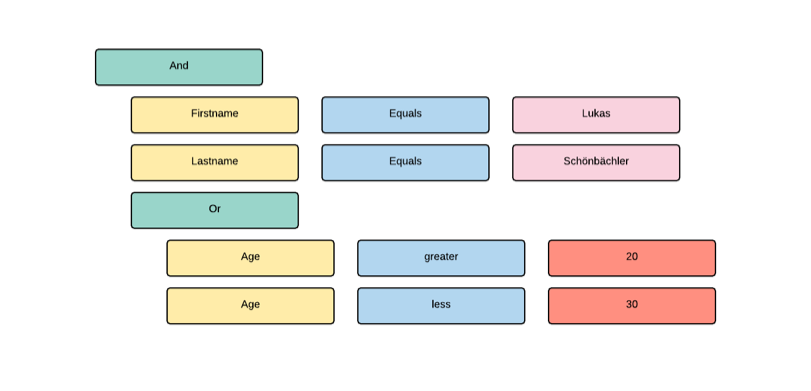
\includegraphics[width=1.0\textwidth]{criteria}
\end{center}
\caption{Criteria tree}
\label{fig:criteria}
\end{figure}

\colorbox{green!30}{   } And / Or: These are Criterias which are non-leaf nodes. They allow to add additional Criterias below (group them)\\
\colorbox{blue!30}{   } Equals / greater / less: Criterias which are leafs, they always evaluate to either true or false\\
\colorbox{yellow!30}{   } Fields / Parameters: Defines to which field value or parameter value the criteria is applied to\\
\colorbox{pink!30}{   } Values: Define which values will be passed to the criteria to evaluate if the result is true or \\
\colorbox{red!30}{   } false. They differ in color to point out that there are different input types such as string or integer. Depending on the type, different Criterias can be chosen (i.e. greater is just available to numeric types). It is possible to use parameters as values by using their placeholder [!PARAMETERNAME] .\\
\\
A tree structure always has one root and therefore always evaluates to one value: true or false. Depending on the outcome of the tree evaluation, the action either will be executed or otherwise the process will end at this point.

\subsubsection{Actions}
If the filter is being evaluated to true, the action will be executed. Possible actions are: sending an E-Mail, SMS, WhatsApp, Push Notification, calling another REST service or even execute another recipe. Depending on the selected action, different configuration fields will show up. I.e. if you select Email as an action, you have to enter a valid email address, a subject and a message body. To improve usability, we validate we provide a WYSIWYG\cite{tinymce} editor with a plugin where you can directly insert all available placeholders. All used parameters are validated by their field types.\\
When the action is triggered, all used fields are processed and all placeholders are replaced by the actual data. After this, the action will be executed and the process is done.

\subsection{Architecture overview}
All these parts together behave in the following matter:\\

\begin{figure}[H]
\begin{center}
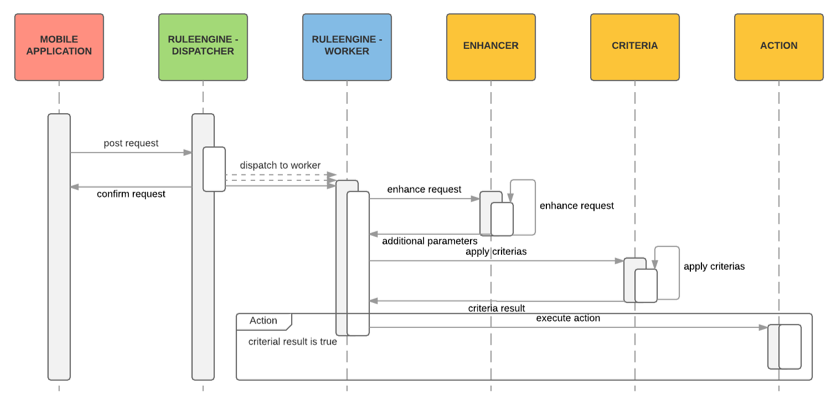
\includegraphics[width=\textwidth]{ruleengine_dispatch_process}
\end{center}
\caption{Rule engine dispatch process}
\label{fig:ruleengine_dispatch_process}
\end{figure}

The mobile application fires a trigger. The dispatcher receives the request, validates the parameters, loads all subscribed recipes, creates a new task for each recipe, dispatches it to the worker queue and confirms the request. An idle worker pulls the next task out of the queue and starts processing it by first adding and processing all enhancers, evaluating the criteria and eventually executing the action in order to complete the process.

\subsection{Logging}

Since the whole process works in the background by either periodic tasks or in an asynchronous submission, there is no direct channel back to the process initiator. Therefore, it is necessary to have a thread safe logging functionality which reveals errors or wrong configurations as soon as they show up. Therefore, we log at different stages in the chain. Generally speaking, we log whenever a component successfully finished its process.\\

We do not have control over the concrete implementations of the components (trigger, enhancer, action), therefore it is in the developer's responsibility to take care about logging potential errors and log them reliable.\\

\begin{figure}[H]
\begin{center}
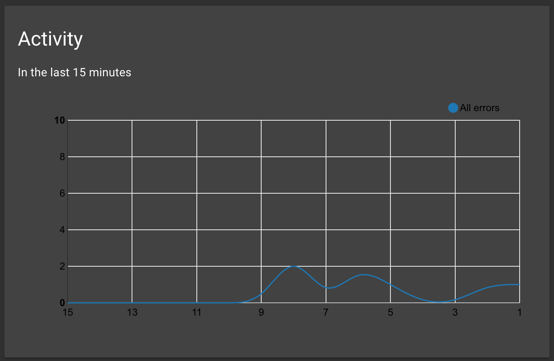
\includegraphics[width=1.0\textwidth]{dashboard_activity}
\end{center}
\caption{Dashboard widget activity}
\label{fig:dashboard_activity}
\end{figure}

In the dashboard we provide two different widgets, one for activity and one for the logs. Both widget display real-time data of the logging component, which means, whenever a log is written, it directly shows up in the interface. This is realized through a web sockets connection to the server. The activity widget shows the usage of the activity of active recipes within the last 15 minutes. The log widget displays more detailed information divided into component, priority, severity and message.

\begin{figure}[H]
\begin{center}
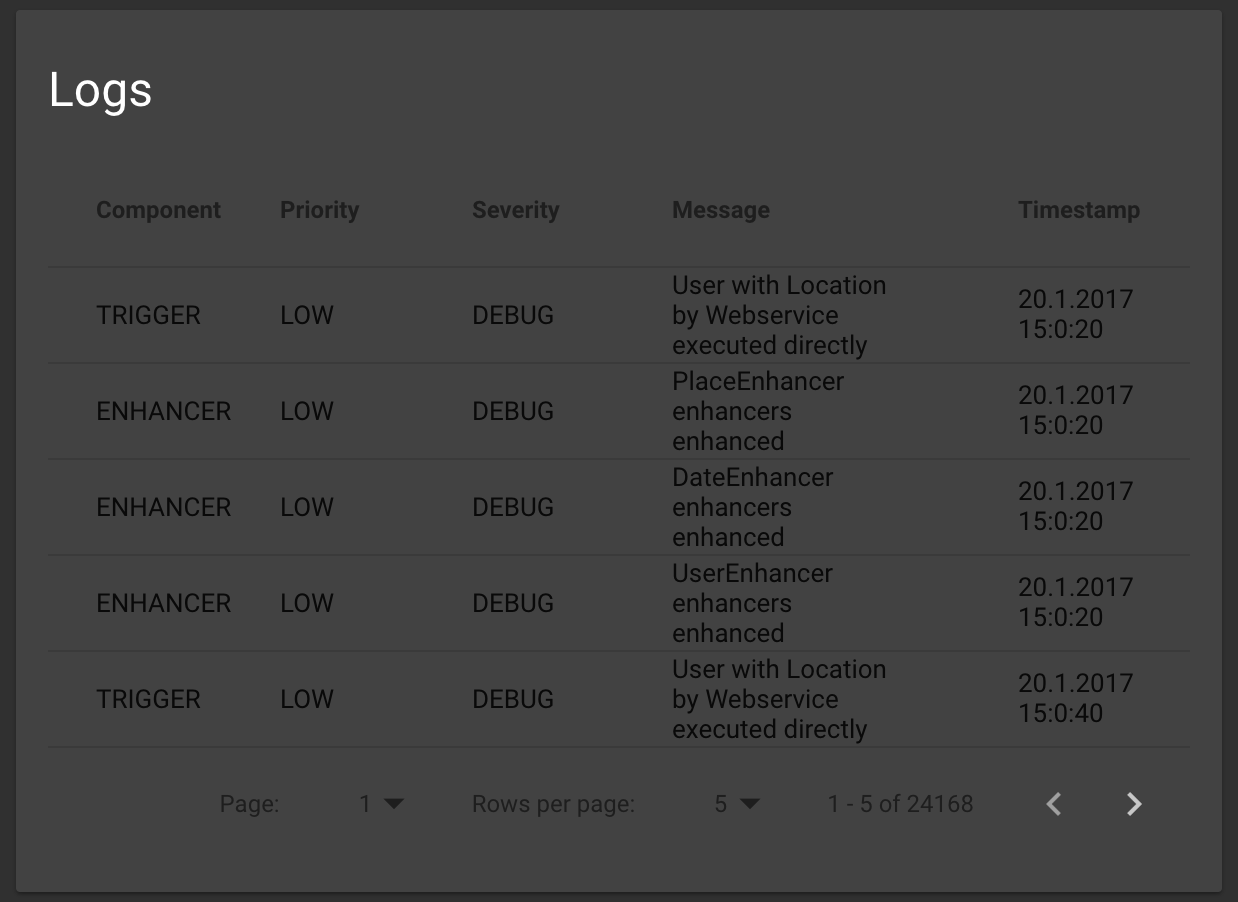
\includegraphics[width=1.0\textwidth]{dashboard_logs}
\end{center}
\caption{Dashboard widget logs}
\label{fig:dashboard_logs}
\end{figure}

\subsection{Extensibility}
One of our biggest advantages with the current architecture is easy to extend. Most additional features can be delivered with only a few lines of code. One only must define which input parameters are needed, pull his additional information or execute his action and return the result. To extend the solution, just look at the code interfaces.

\subsection{Technical limitations}
\subsubsection{Performance}
Currently, the solution is not optimized for performance. Since it is highly scalable due to the queue / worker architecture, this limitation can be resolved by just connecting more worker clients to the pool, but in case the business idea would be successful, other solutions should be considered first. The two biggest potential optimizations are:\\
\begin{itemize}
  \item Remove unused enhancers: Currently all possible enhancers are added to the recipe even though most of the time not all parameters are used. When saving the recipe, all configuration data should be scanned for placeholders. Placeholders which are available but not found in this configuration data should be collected - enhancers which do provide this unused data can be removed.
  \item Improved cron scheduling: Currently all recipes are loaded once a minute to evaluate the cron string in order to check if the cron needs to be executed. There exist certainly more efficient scheduling mechanism than this.
\end{itemize}

\subsubsection{Dependency injection and Single table inheritance}
Unfortunately, the dependency injection isn’t working in the same way we knew it from Java and Spring Boot. This is due to the fact that Django does not support Single Table Inheritance even though it would be possible by our architectural design. Therefore, whenever a new concrete implementation is added, the migration file has to be generated and new tables are generated. The service then must be restarted to load the new schema. We did some research on this topic, but the solutions are more or less “hacky”. We are confident, that there is a clean solution to this problem, but more research would be needed to resolve this limitation.

\newpage
\section{Reflection}
\subsection{Technology}
We both were completely new to Django or Python in general. Because of this, it was a challenge in the beginning. When we started, we did not have a working python development environment. The larger the project grew, the more problems we ran into. But with the help of virtual environments and fixtures, we eventually managed to deal with this kind of issues. With the help of the first steps tutorial (which is very well written), success was achieved early on. The generated admin backend for the entities is good as long as you just need CRUD functionality.\\

Unfortunately for the rule engine, this was not sufficient to make an intuitive GUI. We considered using various frameworks (including Angular 2, which was still early beta) and ended up using Angular 1.5 with Typescript. It's hard to say if it was a good or a bad decision, since we often run into problems, but managed to overcome all of them in the end. Looking back, we probably would use Angular 1.5 again, but without the addition of Typescript.\\

We started developing the application with Ionic 2 very early on. Except of the geofencing part, there were no surprising occurrences at all. Even though Ionic 2  just released in RC0 when we started, the development process was clear and uncomplicated and simple. The hardest thing was debugging, especially when it comes to hardware related stuff like geolocation. But after all, the decision to implement the app with Ionic was a success story.

Generally speaking, we have learned a lot about:

\begin{itemize}
  \item Python (including virtual environments)
  \item Django (models, views, rest framework, fixtures)
  \item Celery (python distributed task queue)
  \item Angular (Typescript with Angular 1.5, components)
  \item Typescript
  \item Cordova plugins/Geofencing (especially their limitations in regards of context / code injection)
  \item Ionic 2
  \item LaTeX
\end{itemize}

\subsection{Architecture}
The business application backend part was straightforward since we just needed standard functionality. All the customization were done within the frameworks specification, without the need of custom functionality beside the business rules.\\
\\
The rule engine architecture was the most interesting and challenging part. We have never designed something similiar to this before. During this process, we have learned a lot about design patterns (i.e. the usage of the composite pattern) and design by contract. If we would start from the beginning again, we probably would aim for an even more generic approach, where each component is just one step, where it is not longer necessary to distinguish between a trigger, enhancer or something else. This most probably would make the UI more complex, but it would give the customer even more control over their customizable processes.
\newpage



\newpage
\begin{appendices}
Below you will find various logins to the following backends:\\
\\
\textbf{Django Admin Backend}\\
https://ip5.sook.ch/admin\\
\\
\textbf{Rule engine}\\
https://ip5-ruleengine.sook.ch/app/\\

\textbf{Superuser}\\
Username: admin@skiuber.com
Password: fhnw\\

\textbf{Organizations/Staff/RuleEngine}\\
Username: org1@skiuber.com
Password: fhnw\\

\textbf{App}\\
Username: user@skiuber.com
Password: fhnw\\

\textbf{Repositories}\\
Username: jluthiger\\
Password: fhnwfhnw22\\
\\
https://git.ernst.to/fhnw/ip5-backend\\
https://git.ernst.to/fhnw/ip5-frontend\\
https://git.ernst.to/fhnw/ip5-ruleengine-frontend\\


\textbf{Endpoints}\\
All endpoint urls are saved in a postman collection to test the rest service. The collection is attached.\\

\textbf{Db-Schema}\\

\begin{itemize}
  \item api-diagram.jpg
  \item ruleengine-diagram.jpg
\end{itemize}

\textbf{Android App}\\

\begin{itemize}
  \item android-debug.apk
\end{itemize}
\newpage
\textbf{Postman collection}\\


\begin{itemize}
  \item ch.fhnw.ipv5.backend.postman\_collection.json
\end{itemize}



\newpage
\listoffigures
\newpage



\begin{thebibliography}{9}
\bibitem{django} 
First steps into Django
\\\texttt{https://docs.djangoproject.com/en/1.10/intro/tutorial01/}

\bibitem{ionic2} 
Ionic 2 Documentation and Available Components
\\\texttt{https://ionicframework.com/docs/}

\bibitem{virtualenv} 
How to setup a virtual environment in python
\\\texttt{http://docs.python-guide.org/en/latest/dev/virtualenvs/}

\bibitem{context-aware} 
Ozgur Yurur and Chi Harold Liu, "Generic and Energy-Efficient Context-Aware Mobile Sensing"
\\\texttt{http://noeticforce.com/mobile-app-development-cordova-vs-react-native-vs-xamarin}

\bibitem{ifttt} 
Structure of IFTTT
\\\texttt{http://engineering.ifttt.com/data/2015/10/14/data-infrastructure/}

\bibitem{celery} 
Celery task queue – multi-threaded backend
\\\texttt{http://www.slideshare.net/richleland/celery-the-distributed-task-queue}

\bibitem{google-maps} 
Ionic 2 with google maps api
\\\texttt{https://www.joshmorony.com/ionic-2-how-to-use-google-maps-geolocation-video-tutorial/}

\bibitem{cordova-plugin-geofence} 
Plugin to monitor circular geofences using mobile devices. The purpose is to notify user if crossing the boundary of the monitored geofence.
\\\texttt{https://github.com/cowbell/cordova-plugin-geofence}

\bibitem{phonegap-geofencing} 
Geofencing And Significant Location Change Monitoring Plugin For PhoneGap.
\\\texttt{https://github.com/radshag/PhoneGap-Geofencing}

\bibitem{cordova-plugin-background-geolocation} 
Cross-platform geolocation for Cordova / PhoneGap with battery-saving "circular region monitoring" and "stop detection".
\\\texttt{https://github.com/mauron85/cordova-plugin-background-geolocation}

\bibitem{cordova-background-geolocation-lt} 
The most sophisticated, battery-conscious background location-tracking and geofencing plugin for iOS and Android
\\\texttt{http://www.transistorsoft.com/shop/products/cordova-background-geolocation}

\bibitem{payment-apis} 
Top Payments APIs: PayPal, Square, Stripe and Others
\\\texttt{https://www.programmableweb.com/news/top-payments-apis-paypal-square-stripe-and-others/analysis/2015/03/11}

\bibitem{ionic} 
The top open source framework for building amazing mobile apps.
\\\texttt{https://ionicframework.com}

\bibitem{xamarin} 
Deliver native Android, iOS, and Windows apps, using existing skills, teams, and code.
\\\texttt{https://www.xamarin.com}

\bibitem{react-native} 
Build Native Mobile Apps using JavaScript and React
\\\texttt{https://facebook.github.io/react-native/}

\bibitem{djoser} 
Djoser authentification  library
\\\texttt{http://www.django-rest-framework.org/api-guide/authentication/\#djoser}

\bibitem{ng-translate} 
The internationalization (i18n) library for Angular 2+
\\\texttt{https://github.com/ocombe/ng2-translate}

\bibitem{geofence} 
Thinking about design with geofence
\\\texttt{https://civic.mit.edu/blog/erhardt/thinking-about-design-with-geo-fences}

\bibitem{geofence-android} 
Creating and Monitoring Geofences
\\\texttt{https://developer.android.com/training/location/geofencing.html}

\bibitem{openweather} 
We Deliver 1 Billion Forecasts Per Day
\\\texttt{https://openweathermap.org/api}

\bibitem{tinymce} 
TinyMCE is a platform independent web-based JavaScript HTML WYSIWYG
\\\texttt{https://www.tinymce.com/}


\end{thebibliography}

\newpage

\section{Honesty declaration}

Hereby, I declare that I have composed the presented work independently on my own and without any other resources than the ones indicated. All thoughts taken directly or indirectly from external sources are properly denoted as such.
\newline

\textbf{Signature} \newline


\vspace{0.5 cm} 
\begin{tabular}{p{7cm}p{1.5cm}l}
Windisch, 22.01.2017
\end{tabular}% 
 \vspace{1 cm} 


\includegraphics[]{lukas}\\
Lukas Schönbächler


\includegraphics[]{tobias}\\
Tobias Ernst

\newpage

\end{appendices}

\end{document}
